\chapter{Full-Stack System Implementation}
\label{ch:implementation}

\section{Software Stack Overview}
To provide production-grade operability, the platform is implemented as a full-stack distributed system combining asynchronous Python microservices with a modern React 18 TypeScript web console.

\begin{table}[H]
  \centering
  \small
  \caption{Software stack specifications and core dependencies.}
  \label{tab:software_stack}
  \begin{tabularx}{\textwidth}{l l p{3.2cm} X}
    \toprule
    \textbf{Component} & \textbf{Technology} & \textbf{Version} & \textbf{Role in Architecture} \\
    \midrule
    SDN Controller & Ryu / Eventlet & 4.34 / 0.33 & OpenFlow 1.3 protocol handling \& switch flow tables. \\
    Emulation Layer & Mininet / OVS & 2.3.0 / 3.1 & Linux network namespaces, veth pairs, TC netem queues. \\
    Backend Framework & FastAPI / Uvicorn & 0.110 / 0.28 & Asynchronous RESTful API \& WebSocket telemetry streaming. \\
    Authentication & PyJWT / Passlib & 2.8 / 1.7 & Stateless HMAC-SHA256 JWT security layer. \\
    Machine Learning & Scikit-Learn & 1.4.1 & Random Forest model training, inference, and serialization. \\
    Agent Framework & LangGraph / LangChain & 0.4.37 / 0.3.14 & Cyclic state machine, tool bus, and agent orchestration. \\
    Frontend Framework & React / TypeScript & 18.2 / 5.4 & Reactive UI, component hierarchy, and strict type safety. \\
    Build Tooling & Vite / Rollup & 8.3.2 / 4.14 & Fast HMR development server and production bundler. \\
    \bottomrule
  \end{tabularx}
\end{table}

\section{Backend Architecture: FastAPI and WebSocket Streaming}
The backend service (\texttt{future/api/main.py}) runs on Uvicorn with an asynchronous event loop listening on port 8000. It mediates between the Ryu controller, the LangGraph agent, and connected frontend web clients.

\subsection{WebSocket Real-Time Telemetry Stream}
Rather than requiring web clients to poll HTTP endpoints continuously (which wastes bandwidth and causes rendering stutter), the backend establishes a persistent WebSocket channel at \texttt{/ws/telemetry}.
\begin{lstlisting}[language=Python,caption={FastAPI WebSocket telemetry broadcast loop.}]
@app.websocket("/ws/telemetry")
async def websocket_telemetry(websocket: WebSocket):
    await websocket.accept()
    try:
        while True:
            # Poll latest switch counter deltas and link states
            payload = get_live_telemetry_snapshot()
            await websocket.send_json(payload)
            await asyncio.sleep(0.5)  # 2 Hz broadcast rate
    except WebSocketDisconnect:
        pass
\end{lstlisting}
Every 500\,ms (2\,Hz), the broadcaster packages link rates, port dropped packet counts, current bottleneck status, active routing mode, and ML hazard probabilities into a lightweight JSON payload and pushes it to all connected browser sessions.

\subsection{Thread-Safe Global State Management}
Because Ryu executes in its own greenlet event loop while FastAPI operates on an asyncio event loop, communication between the controller and the API uses thread-safe memory primitives:
\begin{lstlisting}[language=Python]
class SharedProjectState:
    def __init__(self):
        self._lock = threading.Lock()
        self.routing_mode = "ml_aware"
        self.active_topology = "diamond"
        self.detour_active = False
        self.latest_telemetry = {}
        self.verify_state = {"status": "IDLE", "passed": False}
\end{lstlisting}

\section{Frontend Architecture: React 18 and Canvas Rendering}
The frontend console (\texttt{future/dashboard/react-app}) is a single-page application built with React 18, TypeScript, and Vite. It provides real-time topology visualization, link utilization strip charts, an agent interaction modal, and an empirical research report view.

\subsection{Dynamic Topology Visualizer with Perspective Modes}
The network canvas renders switches, hosts, and interconnecting links via scalable vector graphics (SVG). The visualizer supports three distinct projection modes:
\begin{enumerate}
  \item \textbf{2D Blueprint Mode}: Clean orthogonal layout with color-coded link utilization gradients:
  \begin{itemize}
    \item Green ($\le 50\%$ load): Healthy operating band.
    \item Cyan/Amber (50--80\% load): Elevated traffic.
    \item Hazard Crimson ($>80\%$ load): Critical congestion threshold with pulsing particle animations.
  \end{itemize}
  \item \textbf{3D Perspective Isometric Mode}: 3D isometric projection with adjustable tilt, azimuth, and depth extrusion.
  \item \textbf{3D Topdown Plan Mode}: Planar projection optimized for high-density 11-node WAN layouts.
\end{enumerate}

\begin{figure}[H]
  \centering
  \begin{subfigure}[b]{0.48\textwidth}
    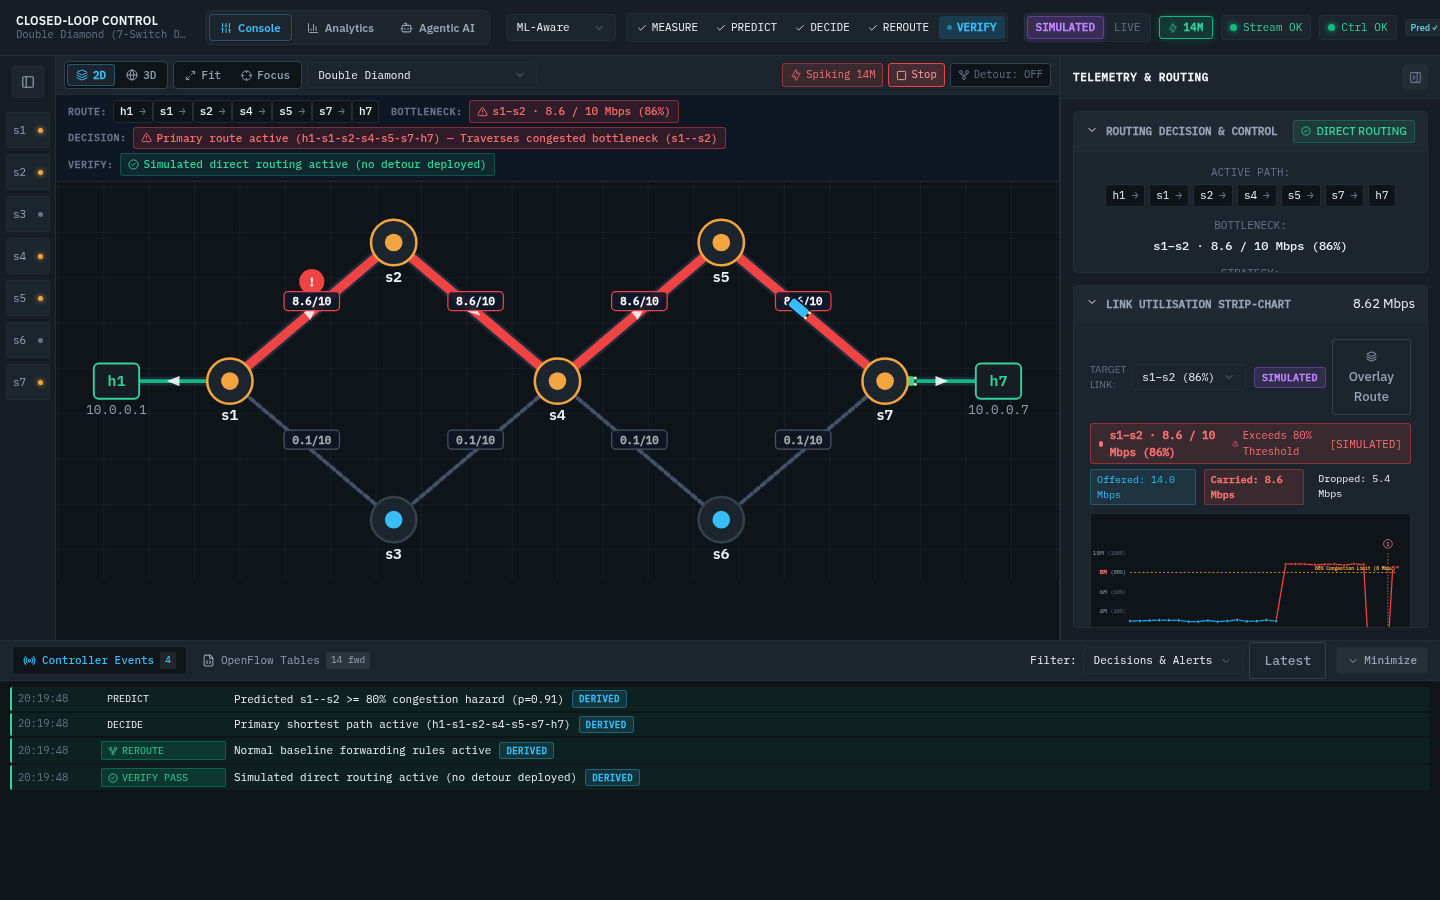
\includegraphics[width=\textwidth]{results/snapshots_ui_fixes/frontend_canvas_congested.png}
    \caption{Active link congestion spike on primary link $s_1 \leftrightarrow s_2$.}
    \label{fig:ui_canvas_congested}
  \end{subfigure}
  \hfill
  \begin{subfigure}[b]{0.48\textwidth}
    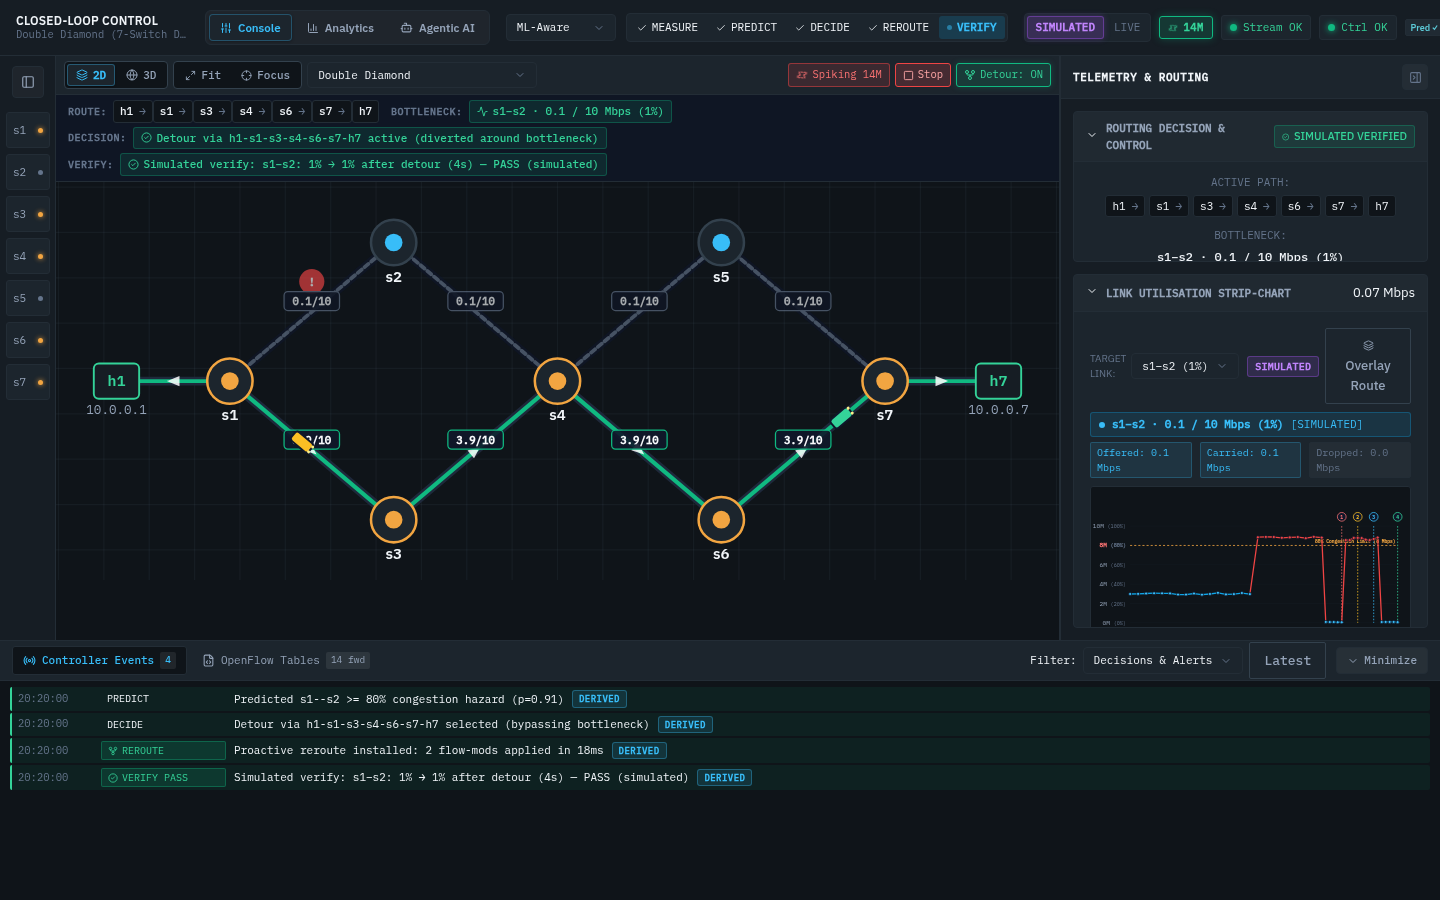
\includegraphics[width=\textwidth]{results/snapshots_ui_fixes/frontend_canvas_detoured_pass.png}
    \caption{Active detour reroute relieving bottleneck link.}
    \label{fig:ui_canvas_detour}
  \end{subfigure}
  \caption{Interactive SVG topology canvas demonstrating live congestion spike and verified detour bypass.}
  \label{fig:canvas_states}
\end{figure}

\subsection{Autonomous Agent Modal Interface}
The LangGraph agent is controlled via an interactive modal (\texttt{AgentModal.tsx}). Operators can interact with the agent using natural-language chat or one-click action pills:
\begin{itemize}
  \item \texttt{[🔥 Create Congestion (14M)]}: Triggers an instant 14\,Mbps traffic spike on the active bottleneck link.
  \item \texttt{[⚡ Fix Congestion]}: Initiates the LangGraph 5-stage closed-loop mitigation workflow.
  \item \texttt{[🔍 Audit Telemetry]}: Prompts the agent to inspect port counters and report status.
\end{itemize}

The modal displays an execution pipeline trace showing live checkmarks across the five stages (\textit{Monitor} $\to$ \textit{Analyze} $\to$ \textit{Plan} $\to$ \textit{Act} $\to$ \textit{Verify}) with execution timestamps.

\section{Publication Markdown Document Viewer (\texttt{RESULTS.md})}
To provide full transparency into empirical data, the frontend includes a dedicated research report viewer (\texttt{MarkdownReportView.tsx}). 

The component parses raw Markdown from \texttt{results/RESULTS.md} and dynamically formats:
\begin{itemize}
  \item Monospace statistical tables with sticky headers.
  \item Verdict badges: \texttt{Best Observed} (blue), \texttt{Separated (p < 0.05)} (green), and \texttt{Overlapping 95\% CI} (muted slate).
  \item Dataset provenance alerts displaying the exact backing files and run counts.
  \item Client-side Copy and Download buttons allowing one-click export of the raw evaluation report.
\end{itemize}

\begin{figure}[H]
  \centering
  \includegraphics[width=0.88\textwidth]{analytics_markdown_report_tab.png}
  \caption{Empirical Markdown Report viewer rendered in the frontend console, presenting statistical hypothesis tests and non-overlapping confidence intervals.}
  \label{fig:ui_markdown_report}
\end{figure}
